\subsection{Muon System}

The forward muon arm has been described in ~\cite{Aamodt:2008zz} . It consists of a
composite absorber ($\sim 10\ \lambda_{int}$), made with layers of
both high- and low-Z materials starting 90 cm from the mean
interaction point, a large dipole magnet with a 3 Tm integrated field
placed outside the L3 barrel magnet, and ten planes of very thin, high
granularity, cathode pad tracking stations. A second muon filter
($\sim 7\ \lambda_{int}$ of iron) at the end of the spectrometer and
four planes of Resistive Plate Chambers are used for muon
identification. The spectrometer is shielded by a dense conical
absorber tube, of about 60 cm outer diameter, which protects the
chambers from secondary particles created in the beam pipe.

The increase of luminosity of the LHC after LS2 requires an upgrade of
the front-end and read-out electronics on both muon
tracking and muon identifier subsystems.


\subsubsection{Muon Tracking}

The Muon Tracking Chambers (MCH)~\cite{Aamodt:2008zz} was operated
during LHC run~1 and run~2. It is based on 156 multi-wire proportional
chambers with cathode pad readout, the so called Cathode Pad Chambers with more than
one million electronic channels. 
The system consists of 5 tracking stations, each of which is composed of 2
chambers. Because of the different sizes of the stations, (ranging from few square metres for station 1 to more than 30 m$^{2}$  for station 5) two different designs were adopted. The first two stations are based on a quadrant structure ~\cite{Peyre}, with the readout
  electronics distributed on their surface (see Figure ~\ref{quad+slat} (Left) ). Four independent quadrants constitute one chamber. For the larger stations (3 to 5), a slat architecture ~\cite{Cicalo} was chosen (see Fig. ~\ref{quad+slat} (Right)). The maximum
  size of a slat is 40 $\times$ 240 cm$^{2}$ and the electronics are mounted on the top and bottom part of
  each slat. Slats are mounted on a support to constitute one
  half-chamber. One half-chamber consists of 9 slats for station 3,
  and 13 slats for stations 4 and 5. The tracking system
  covers a total area of about 100 m$^{2}$. 

\begin{figure}[h]
  \centering
  \includegraphics[width=.45\textwidth]{mch/quadrant.png}
  \hspace{0.05\textwidth}
  \includegraphics[width=.45\textwidth]{mch/slat.png}
   \caption[Tracking system layout]{Left: Layout of station 2 of the tracking system; the readout electronics is distributed on the surface of a quadrant. Right: Layout of stations 4 and 5 of the tracking system; the readout electronics are mounted along the top and bottom edge of the slats.}
  \label{quad+slat}
\end{figure}

Due to the increase of luminosity of the LHC after LS2, the front-end
and the readout electronics have been upgraded, keeping the detectors
unchanged.

The electronics can run either in trigger or in our default dead time free continuous
mode. The data flow readout scheme is shown in
Fig.~\ref{readoutscheme}. The Front-end Cards (FEC) send continuously words through an electrical link at 80 Mbit/s to the SOLAR
read-out board which connects to the Concentrator Readout Unit (CRU)
through GBT optical link at 3.2 Gbits/s.

\begin{figure}[h]
  \centering
  \includegraphics[width=1\textwidth]{mch/readoutscheme.pdf}
     \caption[Tracking readout scheme]{ The Muon Tracking readout scheme}
  \label{readoutscheme}
\end{figure}

\paragraph{The DualSAMPA front-end electronic cards\\}

The front-end electronic cards, called DualSAMPA, host 2 chained SAMPA chips (
see chapter 3.2) of 32
channels each and 3 low voltage regulators. Since the detectors are not
changed, the dimensions and the layout of the connectors for the DualSAMPA cards on the
electronic PCBs remain the same as for the previous FEC. Moreover, two
types of cards were produced, each with the same functionalities but with
different dimensions to cope with the two detector types, quadrant and
slat (see Fig.~\ref{dualsampa}).

\begin{figure}[h]
  \centering
  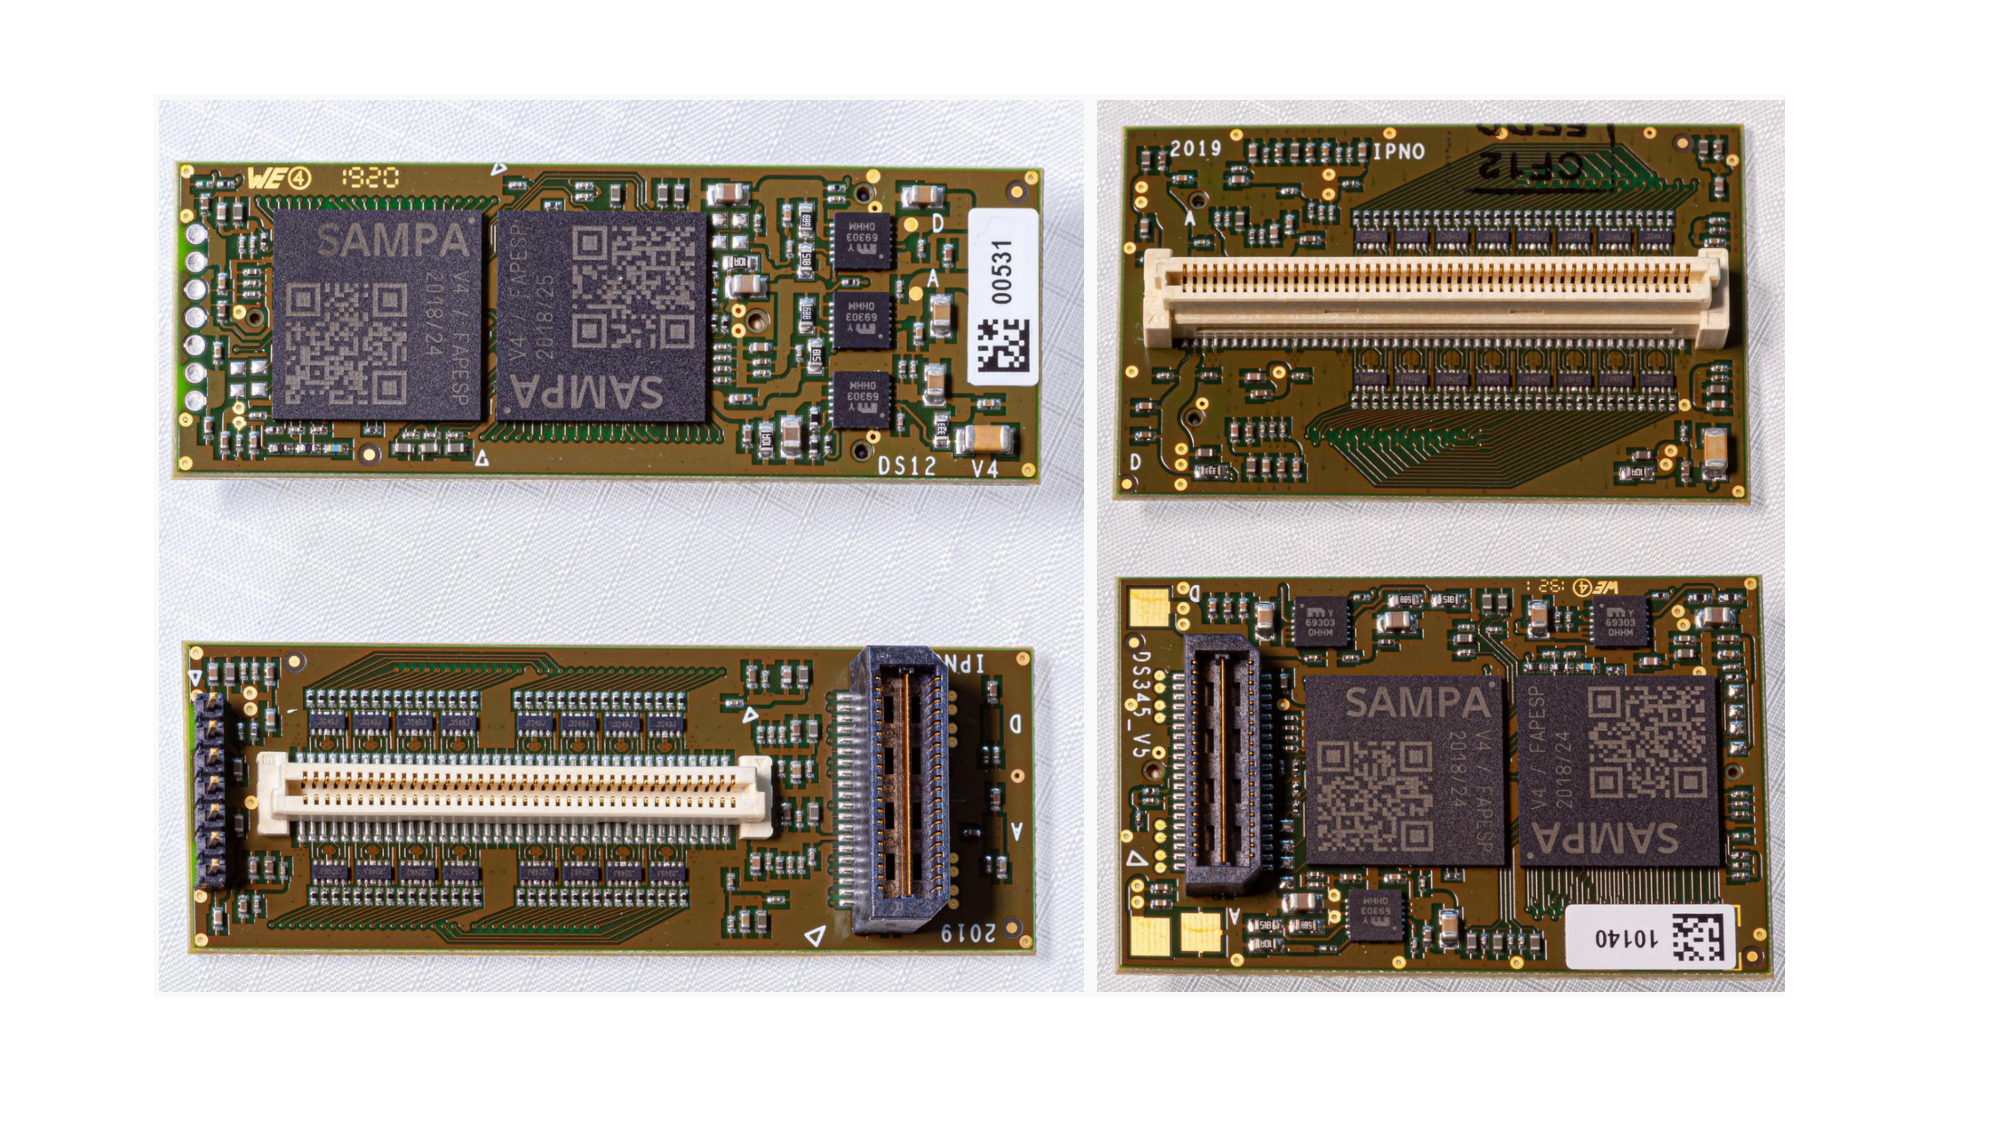
\includegraphics[width=1\textwidth,height=8cm]{mch/dualsampa.pdf}
     \caption[DualSAMPA]{ The two geometries of the DualSAMPA boards,
       with the white connector plug socket on PCB and on the
       other side the black connector connecting to the electrical link. }
  \label{dualsampa}
\end{figure}


Out of the 19300 DualSAMPA produced (11000 DS345 for slats of stations 3,4 and
5 and 8300 DS12 for quadrants of stations 1 and 2), 16900 are
installed in the cavern (9700 DS345, 7200 DS12).

\paragraph{The readout electronic FLEX links and large electronic PCBs\\}

The link between the DualSAMPA and the readout cards consists of a
flexible circuit (FLEX) and a flat ribbon cable for the slats while a
large electronic PCB and a flat ribbon cable is used for the quadrants (see
Figs.~\ref{flex+pcb}(Left) and ~\ref{flex+pcb} (Right)).

\begin{figure}[h]
  \centering
  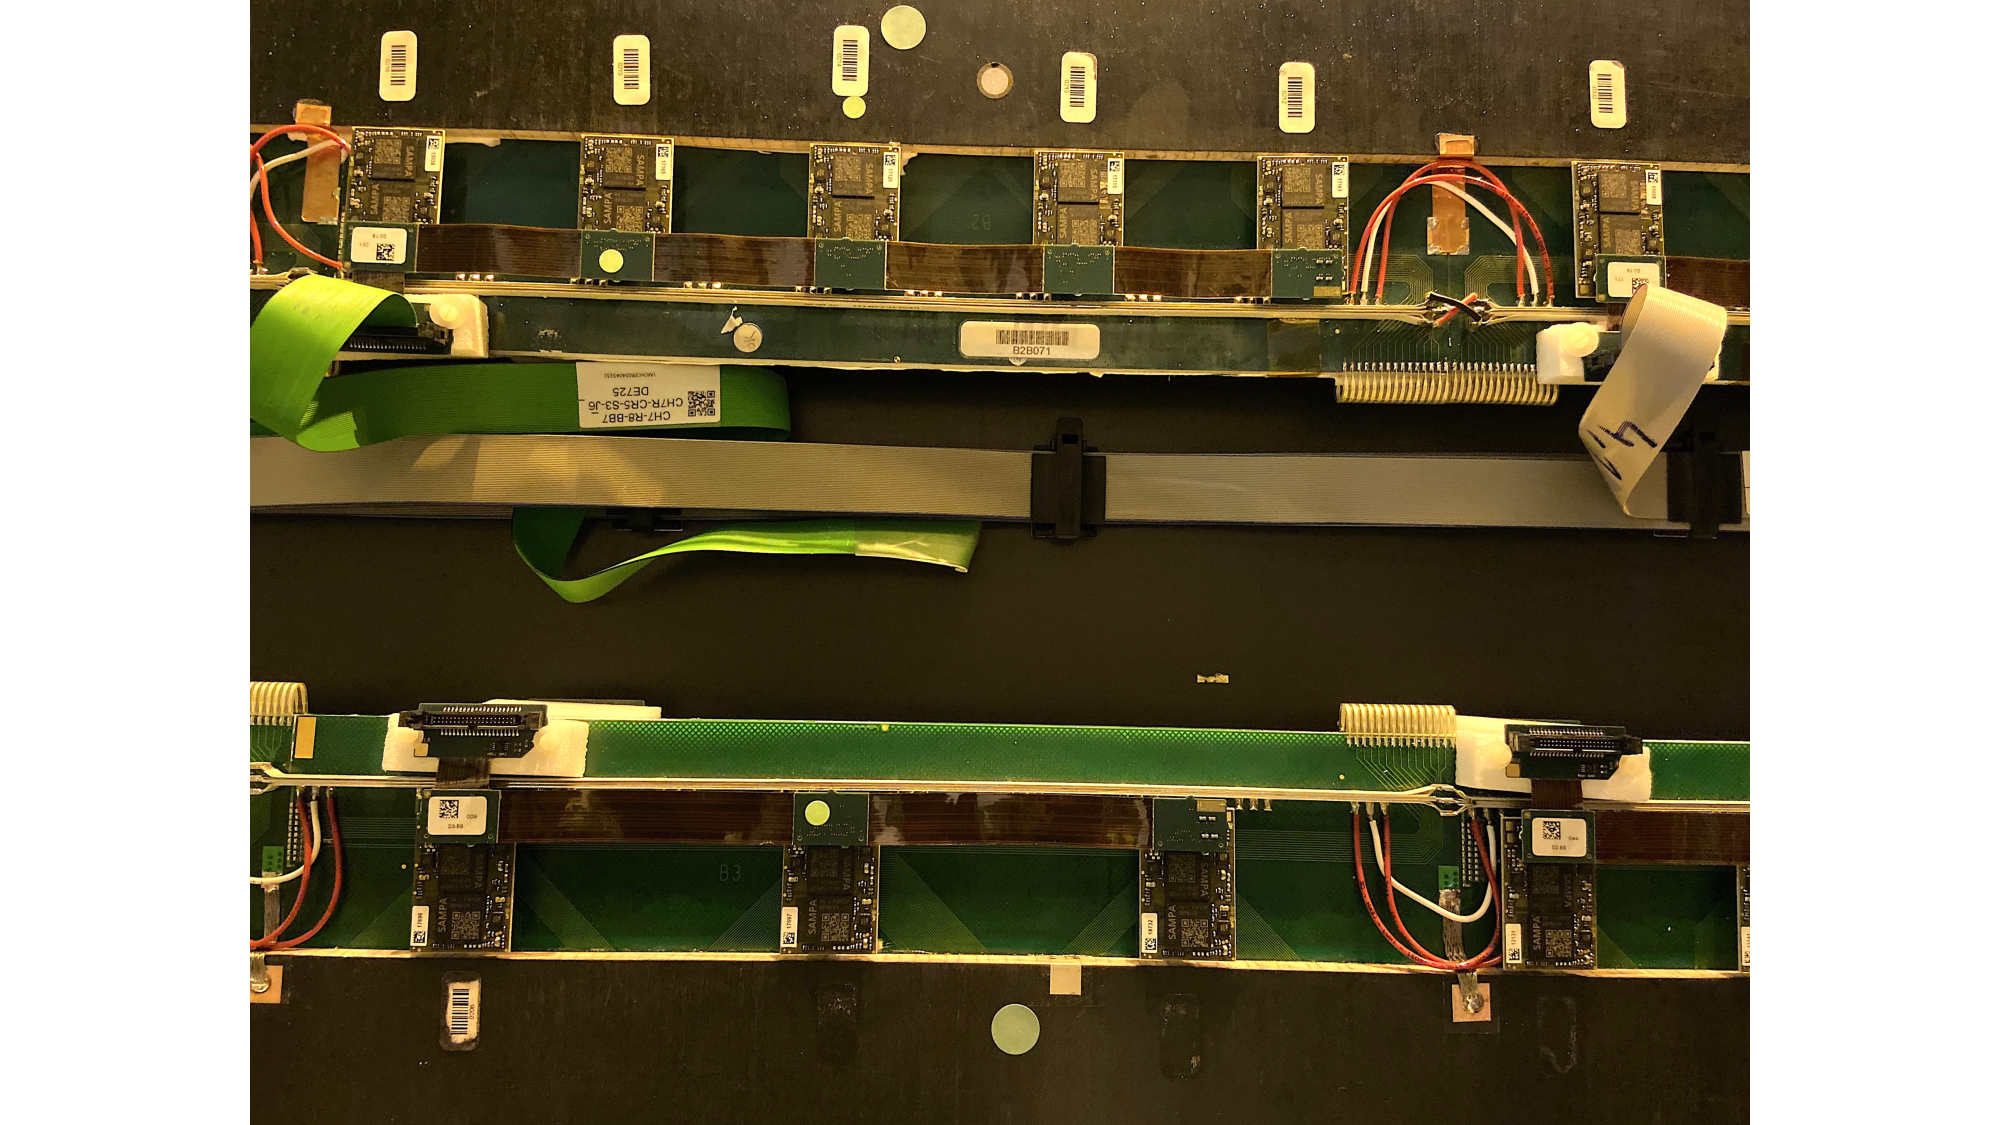
\includegraphics[width=.45\textwidth,height=5cm]{mch/flex.png}
  \hspace{0.05\textwidth}
  \includegraphics[width=.45\textwidth,height=5cm]{mch/largepcb.png}
   \caption[Electronic links]{Left:Flex mounted on a slat connecting 5
     DualSAMPA cards linking through a green flat ribbon cable with the readout
     board. Right:Large electronic PCBs covering the surface of a quadrant.}
  \label{flex+pcb}
\end{figure}

Each DualSAMPA has dedicated data and clock lines while the
trigger lines are daisy chained to feed up to 5 DualSAMPA (see
Fig.~\ref{flexscheme}). A I2C line allows to address up to 5
DualSAMPA. An active buffer was added to the I2C line to insure a
good signal integrity.

More than 3000 FLEX were produced, of 24 different types depending on the number of DualSAMPA
to address, the geometry and pad density; among them 2760 were
installed.
 
\begin{figure}[h]
  \centering
  \includegraphics[width=0.8\textwidth, height= 4cm]{mch/flexscheme.png}
     \caption[FLEX scheme]{ The FLEX scheme}
  \label{flexscheme}
\end{figure}



\paragraph{The SOLAR readout cards\\}
Each FLEX/ribbon cable is plugged into one of the 8 ports of the SOLAR readout
board, allowing this latter to read out up to 40 DualSAMPA boards (see
Fig.~\ref{solarscheme}). The GBTx chip of the SOLAR
board acts as a deserializer of the  signal coming from the DualSAMPA
and a serializer to send the signals from the different FEC to the CRU through GBT optical
links. The SOLAR board hosts also a GBT-SCA chip handling the 8 I2C
command/control lines, one optical transmitter/receiver VTRx and 2
DC/DC FEAST converters. 
 
\begin{figure}[h]
  \centering
  \includegraphics[width=1\textwidth]{mch/solarscheme.png}
     \caption[SOLAR scheme]{ The SOLAR scheme}
  \label{solarscheme}
\end{figure}

The 624 boards produced are placed in 112 custom SOLAR crates, each
one hosting up to 6 boards.


\paragraph{The data flow from SAMPA to the CRU User Logic\\}
In the SAMPA chip, the signal of each electronic channel is amplified with a ~4mV/fC gain,
waveformed with a shaping time of 300 ns, then sampled and digitized at 10 MHz in
a 10-bits ADC and is finally digitally processed with a baseline
correction and a zero-suppression before being formatted. The SAMPA format
consists of data samples from a signal waveform with its time stamp and
size together with a header containing mainly the bunch crossing number, the SAMPA
address and the channel address of the SAMPA chip.

 The signals of the 64 channels of
the two-chained SAMPA chips of a FEC are serialized at 80
Mbits/s (2bits at 40 MHz). The first port of the SOLAR board handles
the first 2 bits of the first DualSAMPA while the second port takes care of the 2 bits of
the second DualSAMPA and so on up linking all 40 ports whihc results in a 4.2
Gbits/s data optical transmission to one input of a CRU. The
electrical and optical links are always sending words, whatever the
type of information (physics data, synchronisation (SYNCH), ...). 

The MCH CRU User Logic (UL) receives data from the 24 GBT links (see description of the CRU in
chapter 6.3), each one handling 40 DualSAMPA channels. For each GBT
link, the UL deserializes the 80 bits, forms the SAMPA
words, remove the SYNCH words and inserts error checks and
condition. The 64 bits SAMPA words contain the payload, the GBT
link identifier, the DualSAMPA channel identifier, and error bits. The
UL then embeds the TTC signals into the stream, constructs
the RDH (Redaout Data Header) and transmits words of 256 bits to the FLP (Front Level
Processor) (see Fig. ~\ref{dataflow} and~\ref{cru-ul}).

\begin{figure}[h]
  \centering
  \includegraphics[width=0.7\textwidth,height=3cm]{mch/dataflow.png}
     \caption[Data flow]{Data flow scheme}
  \label{dataflow}
\end{figure}

\begin{figure}[h]
  \centering
  \includegraphics[width=1\textwidth]{mch/cru-ul.png}
     \caption[CRU Scheme]{CRU scheme}
  \label{cru-ul}
\end{figure}

The $O^2$ processes, carried out on FLPs or/and EPN,  will perfom the decoding of the data
format received from the CRU, the pre-clustering, clustering and tracking. These
will also run the simulations.
During data taking the Quality Control (QC) processes data samples for detector performances
monitoring.



\input{mid}